\subsection{RQ3: generality across corpora and architectures}
\label{sec:rq_generality}

\emph{In short:} the benefit of dropping project vocabulary holds on both
corpora and under every architecture we tried (the Transformer on BigVul
only); the choice of architecture
moves AUC by much less than the choice of node view, but only within the
family of small models we can train from scratch.

Table~\ref{tab:rq3_generality} repeats the main comparison on DiverseVul and
under three further architectures: GAT and GIN (two other message-passing
schemes) and a Transformer encoder over the pre-order node sequence, which uses
no graph edges at all (BigVul only, for cost). Figure~\ref{fig:forest} plots
the gains against the text-only view.

% Generated by experiments/emit_tables.py -- DO NOT EDIT BY HAND.
% Every value is read from experiments/results/*.json.

\begin{table*}[t]
\centering
\caption{RQ3: mean AUC over 10 matched folds for four node views under every
backbone and corpus, and the paired gain of $\kappa$ and of lexical$+\kappa$
over the lexical view (point estimate, 95\% cluster-bootstrap interval,
bootstrap $p$; \emph{n.s.}: interval contains zero).}
\label{tab:rq3_generality}
\resizebox{\linewidth}{!}{%
\begin{tabular}{llrrrrll}
\toprule
Corpus & Backbone & Lexical & Lex$+\kappa$ & $\kappa$ & $\kappa{+}\phi$ & $\kappa$ vs lexical & Lex$+\kappa$ vs lexical \\
\midrule
BigVul & GGNN & 0.506 & 0.592 & 0.691 & 0.687 & $+0.140$ $[+0.096, +0.201]$ $<0.001$ & $+0.074$ $[+0.040, +0.109]$ $<0.001$ \\
BigVul & GAT & 0.507 & --- & 0.673 & 0.654 & $+0.127$ $[+0.085, +0.182]$ $<0.001$ & --- \\
BigVul & GIN & 0.574 & --- & 0.704 & 0.719 & $+0.063$ $[+0.011, +0.142]$ 0.016 & --- \\
BigVul & Transformer & 0.582 & --- & 0.706 & --- & $+0.132$ $[+0.095, +0.171]$ $<0.001$ & --- \\
DiverseVul & GGNN & 0.566 & 0.607 & 0.667 & 0.675 & $+0.111$ $[+0.081, +0.140]$ $<0.001$ & $+0.043$ $[+0.020, +0.066]$ $<0.001$ \\
DiverseVul & GAT & 0.558 & --- & 0.652 & 0.654 & $+0.091$ $[+0.062, +0.120]$ $<0.001$ & --- \\
DiverseVul & GIN & 0.574 & --- & 0.679 & 0.687 & $+0.117$ $[+0.085, +0.148]$ $<0.001$ & --- \\
\bottomrule
\end{tabular}}
\end{table*}


\begin{figure}[t]
\centering
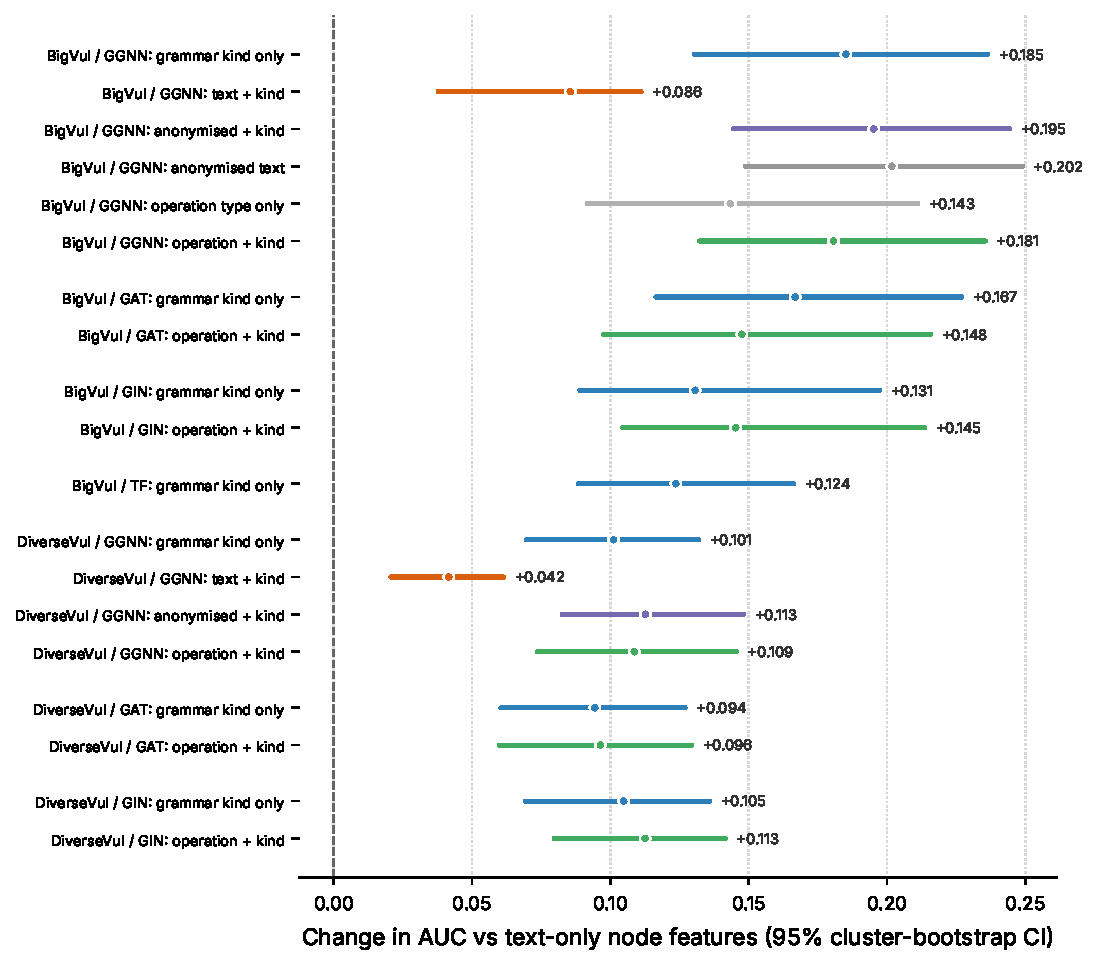
\includegraphics[width=\linewidth]{figures/fig_representation_forest.pdf}
\caption{Change in AUC against text-only node features for each corpus and
architecture, with 95\% cluster-bootstrap intervals over held-out projects.
Intervals that include zero would be marked n.s.}
\label{fig:forest}
\end{figure}

\paragraph{Corpora and message-passing schemes} Under GAT and GIN, and on
DiverseVul, the grammar kind improves on text in every comparison
(Table~\ref{tab:rq3_generality}; for example
\cDvGgnnKindVLexD{} on DiverseVul with the GGNN, \cDvGatKindVLexD{} with the
GAT and \cDvGinKindVLexD{} with the GIN). The gain varies by corpus
(\cBvGgnnKindVLexD{} on BigVul with the GGNN, against \cDvGgnnKindVLexD{} on
DiverseVul).

\paragraph{The architecture claim, narrowed} The earlier submission asserted
that representation matters more than architecture on the strength of three
message-passing networks whose AUCs differed by $0.027$. That evidence cannot
support a claim about architecture in general, and we now state what it does
support. Under a fixed vocabulary-free view the three message-passing
networks (GGNN, GAT, GIN) span \numbvSpreadKind{} AUC on BigVul with the
grammar kind and \numdvSpreadKind{} on DiverseVul; under the text view they
span \numbvSpreadLex{} and \numdvSpreadLex{}. The widest of these ranges is
smaller than the smallest gain of any vocabulary-free view over text
(\numdeltaMin{}), so within this family the node view is a larger lever than
the backbone. The Transformer adds a different inductive bias (no edges); its
AUC is \mBvTfLexAuc{} with text and \mBvTfKindAuc{} with the grammar kind, so
the benefit of the vocabulary-free view is not specific to message passing.
What our evidence cannot show is that no \emph{pretrained} or much larger
architecture would close the gap by itself, and Section~\ref{sec:rq_reference}
shows that a fine-tuned pretrained code model, reading format-normalised source,
beats the vocabulary-free graph views by a small margin.
